\documentclass{article}
\usepackage[utf8]{inputenc}
\usepackage[T1]{fontenc}
\usepackage{amsmath, algorithm, algpseudocode}
\usepackage{tikz}
\usetikzlibrary{shapes.geometric, arrows, positioning}

\begin{document}

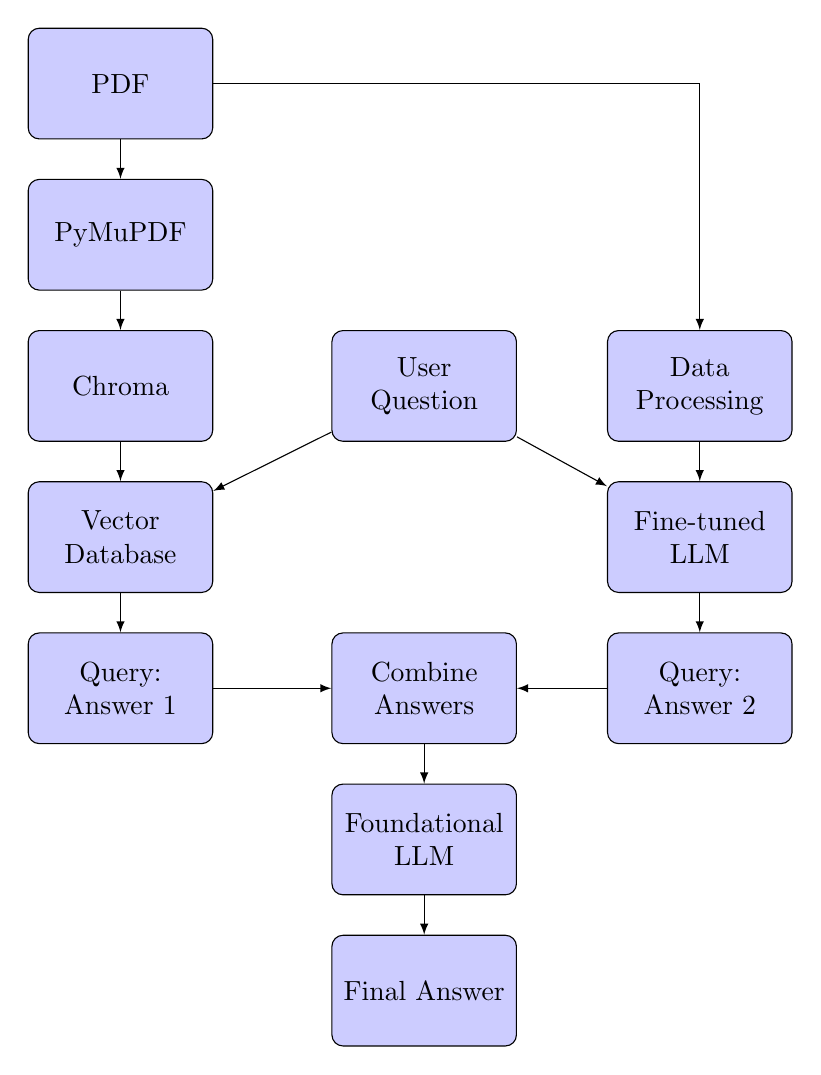
\begin{tikzpicture}[
    node distance=0.5cm and 1.5cm,
    auto,
    block/.style={rectangle, draw, fill=blue!20, text width=6em, text centered, rounded corners, minimum height=4em},
    line/.style={draw, -latex}
]

\node[block] (pdf) {PDF};
\node[block, below=of pdf] (pymupdf) {PyMuPDF};
\node[block, below=of pymupdf] (chroma) {Chroma};
\node[block, right=5cm of chroma] (dataprocess) {Data Processing};
\node[block, below=of chroma] (vectordb) {Vector Database};
\node[block, below=of dataprocess] (finetune) {Fine-tuned LLM};
\node[block, below=of vectordb] (query1) {Query: Answer 1};
\node[block, below=of finetune] (query2) {Query: Answer 2};
\node[block, right=1.5cm of chroma] (userquestion) {User Question};
\node[block, right=1.5cm of query1] (combine) {Combine Answers};
\node[block, below=of combine] (finalmodel) {Foundational LLM};
\node[block, below=of finalmodel] (finalanswer) {Final Answer};

\path[line] (pdf) -- (pymupdf);
\path[line] (pymupdf) -- (chroma);
\path[line] (chroma) -- (vectordb);
\path[line] (pdf) -| (dataprocess);
\path[line] (dataprocess) -- (finetune);
\path[line] (userquestion) -- (vectordb);
\path[line] (userquestion) -- (finetune);
\path[line] (vectordb) -- (query1);
\path[line] (finetune) -- (query2);
\path[line] (query1) -- (combine);
\path[line] (query2) -- (combine);
\path[line] (combine) -- (finalmodel);
\path[line] (finalmodel) -- (finalanswer);

\end{tikzpicture}

\end{document}